\documentclass[a4paper]{article}
% \usepackage[fontsize=13.9pt]{fontsize}
\usepackage[margin=4cm]{geometry}
\usepackage[style=numeric]{biblatex}
\bibliography{citation}
% \documentclass[a4paper]{article}
\usepackage{fontspec}
\usepackage[]{flowfram}
\usepackage{graphicx}
\usepackage{tabularx}
\usepackage{hyperref}
\usepackage{booktabs}
\usepackage{float}
\usepackage{wrapfig}

\ffvadjustfalse

\author{Xiyan Shao}
\title{Towards Unsupervised Few-Shot Text Style Transfer: A Method with Pretrained LM and Style Extractor}
\begin{document}
\maketitle
\section{Introduction}
Responding to changing contexts and audiences, people speak and write in different styles.
A naturally occurring linguistic variation, \textit{style} is defined by a large set of
attributes of texts which includes but is not limited to formality, politeness, diction, and emotion. Text style transfer (TST) is a task in NLP that aims to change certain attributes in the style of a text while preserving its meaning.
A task with a long history, it has significant applications for downstream tasks like machine translation, in which it can help reduce the difficulty of interpreting stylistic texts;
text simplification, in which it translates complicated text for a wider audience; and formality transfer, in which help modify the formality of text for different social contexts. Table \ref{tab:original_and_stylized_text} shows some transfer examples.

However, unlike the well-known success in image style transfer, the progress of text
style transfer has been greatly limited by the discrete nature of text data and, more
crucially, the lack of parallel training data. As identified by many researchers, a
key problem in the TST task is how to develop unsupervised models that can make use
of the abundant unlabeled training data which enabled training huge language models
like BERT, T5, GPT, and so on.

% insert table of two columns, one for original text, one for stylized text
\begin{table}[h!]
\centering
\label{tab:original_and_stylized_text}
\begin{tabularx}{\linewidth}{XX}
Original text & Stylized text \\ \midrule 
(Rude) What the hell is wrong with your attitude? & (Polite) Perhaps the question is more about your attitude.\\
(Positive) Apple's new chip worths it's price. & (Negative) Apple's new chip is to expensive to afford.\\
\end{tabularx}
\caption{Example of text style transfer tasks}
\label{tab:original_and_stylized_text}
\end{table}

\section{Methodology}

In this project, I aimed to leverage large pre-trained language models to approach the
TST task with transformer models. After experimenting with a naive seq2seq model
based on T5 \cite[][]{raffel_exploring_2020} with a language model head and a Generator-Discriminator network that
enables adversarial training \cite[implementing][]{dai_style_2019}, I ended up
developing and training a T5 based conditional generation model with a language model
head and a style extractor encoder which performs much better than the GAN model and appears
more flexible than the naive se2seq finetuning approach. Proposed by Riley et al., this more
recent approach features few-shot tunable targeted restyling and style extraction \cite[]{riley_textsettr_2021}.

\subsection{Model Architecture}

Since the source code is not openly released, from scratch, I implemented a
\texttt{T5ForConditional GenerationWithExtractor} model by extending the vanilla
T5 model from the \texttt{huggingface/ transformers} repository. Following the
TextSETTR model architecture, multiple changes were made (e.g., noise generation
function, extractor specifications, and hyperparameters) to reproduce the paper's
result with limited computational resources. Finally, I achieved a working and
probably the first third-party implementation of T5 based text style extraction model.
The model definition is as follows.

\begin{figure}[H]
    \centering
    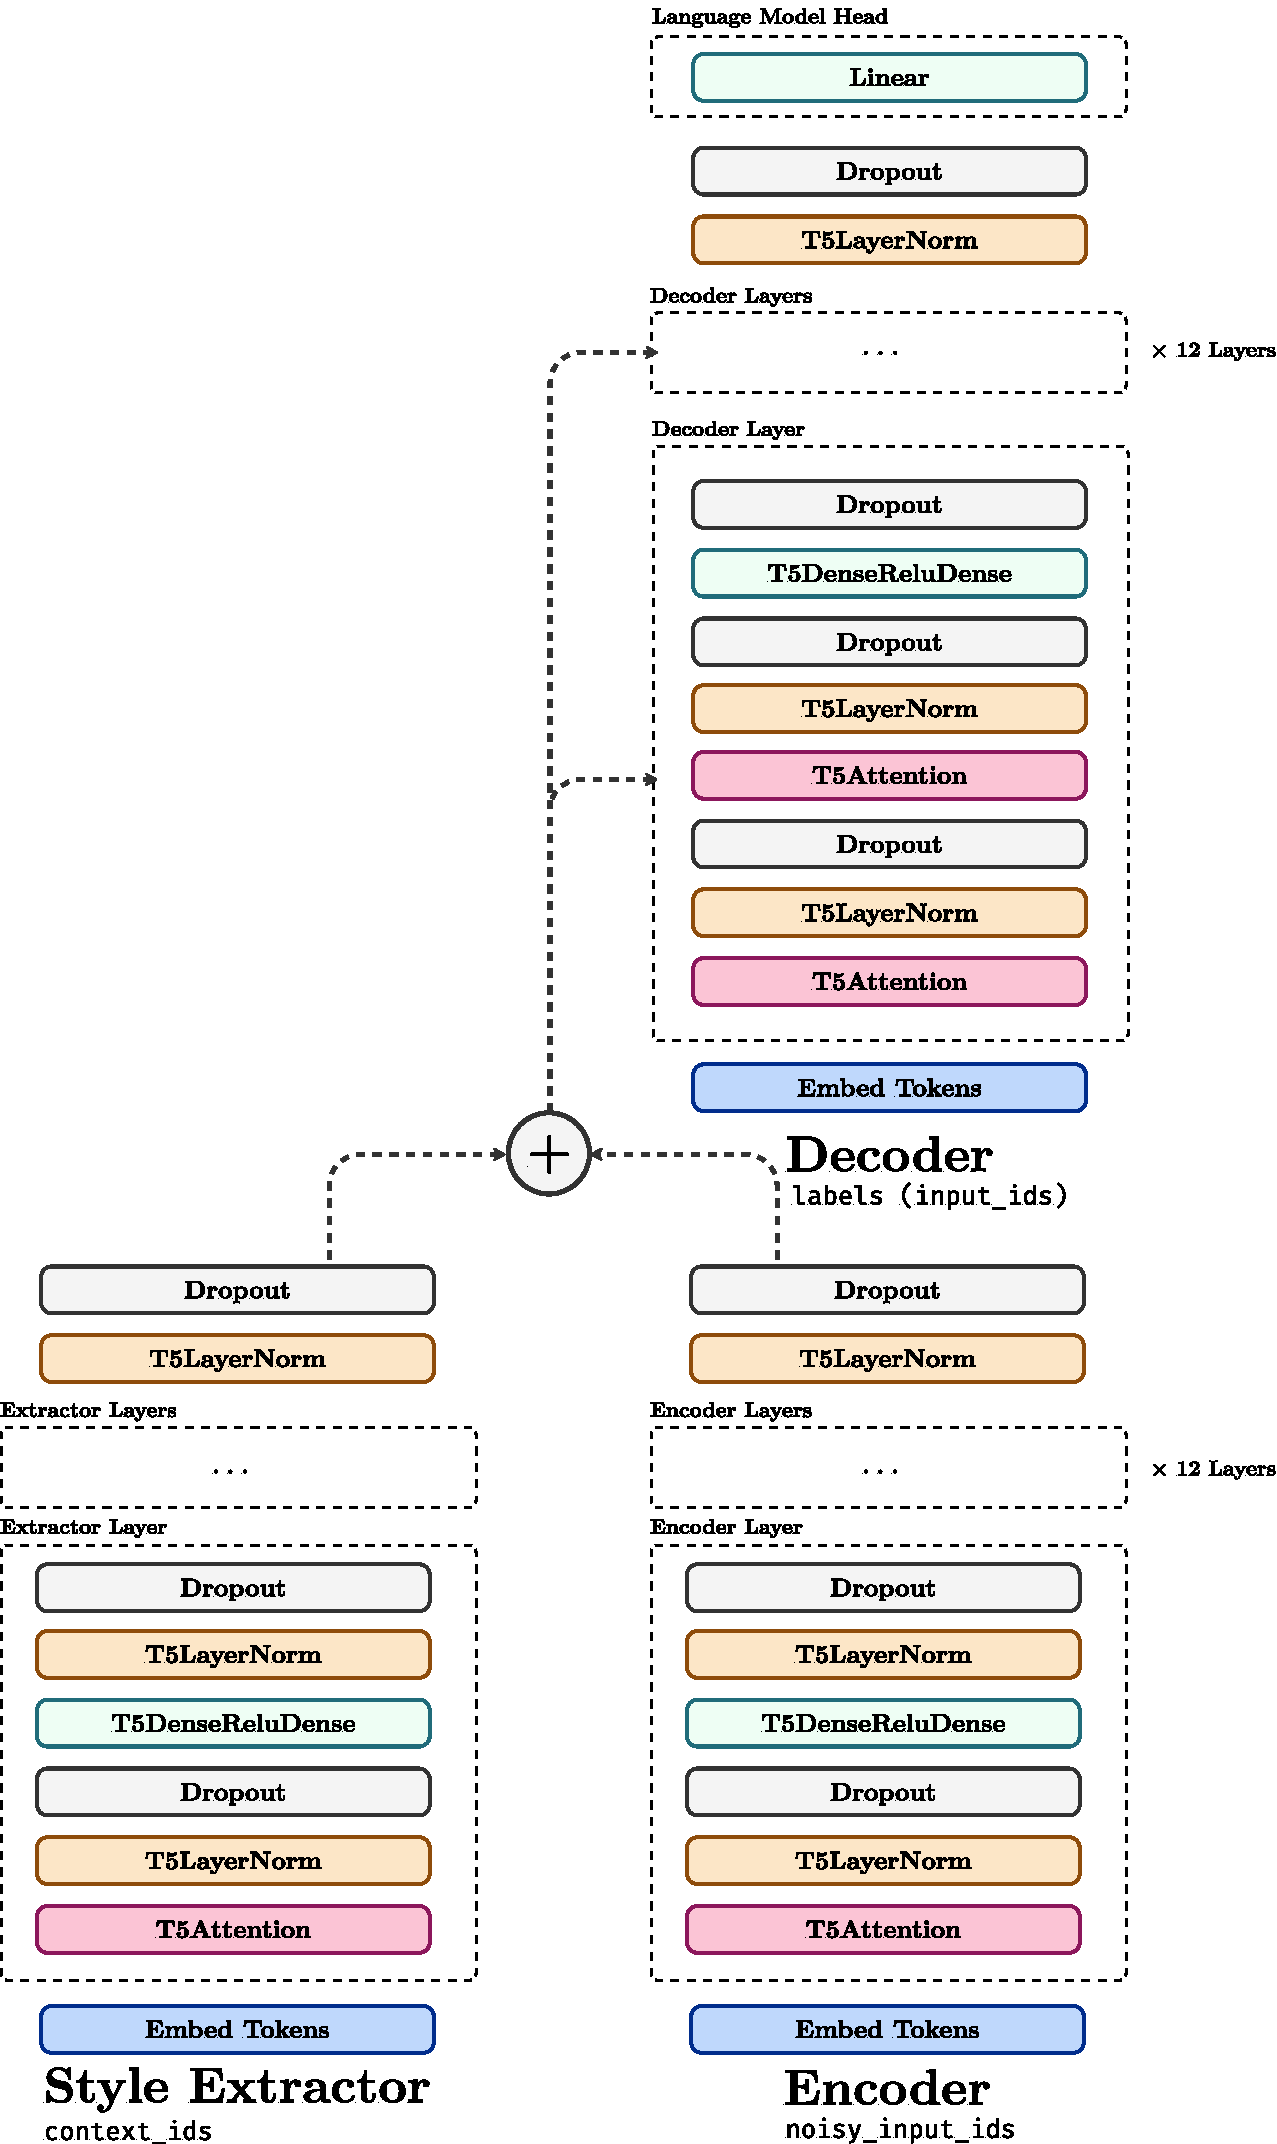
\includegraphics[width=0.7\textwidth]{model_df.pdf}
    \caption{T5ForConditionalGenerationWithExtractor}
    \label{fig:T5ForConditionalGenerationWithExtractor}
\end{figure}

In my implementation, the encoder and decoder are identical to those in the T5-base model, and two more modules are appended to the encoder-decoder network -- a style extractor and a language model head. The style extractor is, in my implementation, a deep copy of the encoder module (weights and biases not tied). Before training, the extractor module is initialized with weights identical to the those of encoder. The language model head is a single layer feed-forward network projecting the hidden states to the vocabulary size. The last hidden states of the encoder and the style extractor are combined via addition and fed into the decoder's attentions. Under the assumption that adjacent sentences in the same context share the same style, the style extractor will be able to extract the style of the context sentence, as facilitated by a noisy reconstruction task. More details about the training/inference process will be discussed in later sections.

\subsection{Data Preparation}
The T5 with style extractor model is trained on a subset of the \href{https://nijianmo.github.io/amazon/index.html}{Amazon Review Data (2018)} dataset. Since the whole dataset is too large, I randomly sampled one million lines from the 5-core sub dataset. The dataset is preprocessed by only taking reviews with $\ge$ 2 sentences, where each sentence has 30 or more characters. I implemented a PyTorch Dataset class to load the dataset and preprocess the data, and for every pair of sentences in the dataset, the first sentence is used as the context and the second sentence the as the input. Eventually, the data preprocessor tokenizes the sentences using the original T5 tokenizer, splits up the training, validation, and testing datasets, and packages all the data loaders into a Pytorch Lightning DataModule for batching and training.

\subsection{Training}
The training of T5ForConditionalGenerationWithExtractor is unsupervised and facilitated by a reconstruction task. I implemented helper functions to add noise to the input sentence (one for adding noisy tokens (40\%) and another one for randomly dropping tokens (20\%)). Like the original paper method, I also employed the Noisy Back Translation technique (same amount as the mechanical noises) to improve the transfer accuracy. Figure \ref{fig:T5ForConditionalGenerationWithExtractor} above shows the data flow of the training process. The preceding sentence tokens are used for the context, and the following sentence tokens with Drop/Add + NBT noise are used as the input IDs. With the training goals being to reconstruct the noisy text based on the context style, the ground true sentences are directly fed into the decoder for a cross-entropy loss atop the linear language model head. For hyperparameters, I used the AdamW optimizer with a learning rate of 1e-3 and Pytorch Lightning's automatic scheduler. The batch size is set to 64, and the maximum number of tokens is set to 32. Since I have access to only one P100 GPU on Google Colab and there are over 332 million trainable parameters, I trained the model for 2 epochs. Hopefully, this is sufficient for a proof of concept.

\begin{figure}[H]
    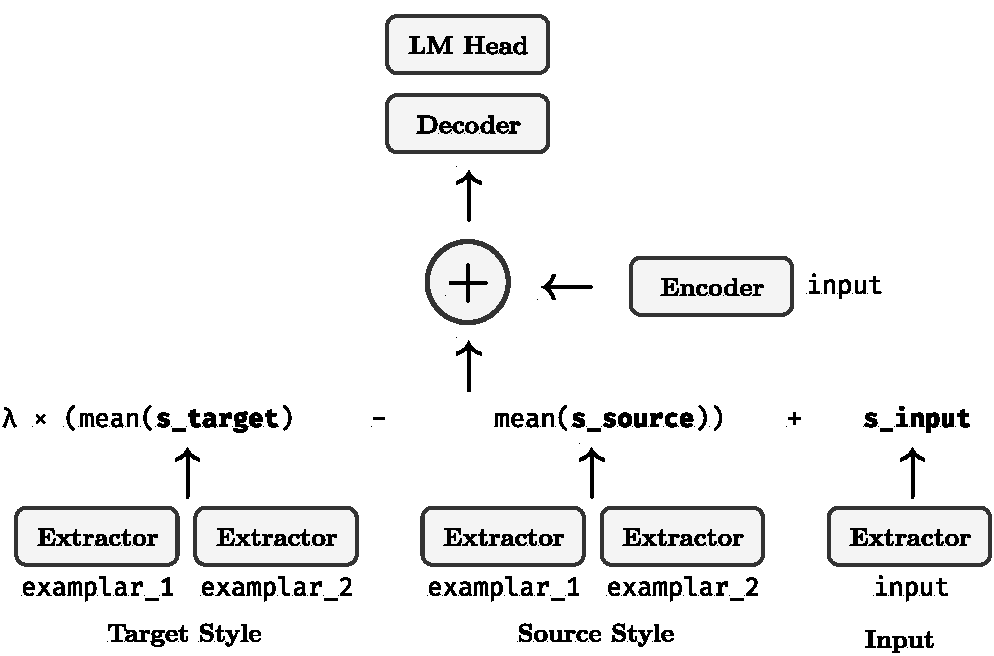
\includegraphics[width=\linewidth]{eval.pdf}
    \caption{Few-shot Inference}
    \label{fig:eval}
\end{figure}

In inference mode, the strategy illustrated in figure \ref{fig:eval} is used to transfer text styles on a few-shot basis. First, we choose a style target style and also a source style similar to the input style. We feed the extractor with exemplars for both styles and get the corresponding style embeddings, and by subtracting the target style embedding from the source style embedding, we get a style vector pointing towards the target style. In this way, by adding the style direction to the extracted input style, we can get the transferred style. The style vector is then summed with the input encoder's final hidden states to get the final embedding, which is to be decoded. After a greedy search for the language model output, we get the predicted output sentence.

\section{Results}

\begin{table}[h!]
    \centering
    \label{tab:result}
    \begin{tabularx}{\linewidth}{XX}
    \midrule[1pt]
    Source  & Result \\  \midrule
     I hereby commit to never purchase anything from this institution in the future. & I'm hereby gonna never buy from this seller again.\\
     I couldn’t figure out what the author was trying to say. & (Formal) I couldn't figure out what exactly the author was trying to say. \newline (Informal) I couldnt figure out what the author was trying to say.\\\midrule[1pt]
     \end{tabularx}

    \begin{tabularx}{\linewidth}{XXX}
    \midrule[1pt]
    Prompt & Emotional & Reserved\\\midrule
    My favorite movie is $\cdots$ & My favorate movie is awesome. My Favorate Movie is amazing! & My favorate movie is the movie which is great.\\
    Please get $\cdots$ & Please get it! & Please get it. Please do get this. \\\midrule[1pt]
    \end{tabularx}

    \begin{tabularx}{\linewidth}{XXX}
        \midrule[1pt]
        Prompt & Negative & Positive \\\midrule
        The product is $\cdots$ & The product is defective. & The product is good The Product is excellent\\
        Apple watch is $\cdots$ & Apple watch is useless. & Apple watch is amazing.\\
        The University of California at San Diego is $\cdots$ & The University of California at San Diego is a dead zone. & The University of California at San Diego is beautiful.\\
        \end{tabularx}
        \caption{Example Results}
        \label{tab:result}
\end{table}

Table \ref{tab:result} shows some results of the model. Towards a qualitative evaluation, I tested the model on several tasks. The first group shows the model's performance in the formal $\leftrightarrow$ informal transfer task, and all the outputs are generated by conditioning on only 3 exemplars for each style. We can observe that the first result is pretty remarkable, and the second result shows the flexibility of transfer directions (target style not necessarily $\ne$ input style) -- for the formal $\rightarrow$ informal direction, notice that it spells \textit{couldn’t} as \textit{couldnt}, a sign of informal language.

The second group of examples shows that besides seq2seq, this model is capable of conditional generation. Provided with prompt and conditioned on only 3 examples in each style category, the generated texts differ by their level of emotion.

Another important task of test style transfer is sentiment transfer. However, it seems like the model is performing poorly on the seq2seq sentiment transfer task (where the model almost always changes a minimum number of words). However, when used in a conditional generation setting, we can see that the outputs are both accurate and consistent. \footnote{For examplars of styles used in the few-shot inference, see the appendix. Positive and negative examplars were sampled (n=100) from the Yelp review polarity dataset.}

Nonetheless, from the example above, one can also see that in some examples the generation accuracy is questionable, and sometimes the generation fluency is not ensured. Notably, the model is prone to repeat itself. This is probably limited by the amount of training data (I only used less than 1/100 of the original dataset) and the insufficient training steps. Contrary to the original paper, I used the t5-base model instead of t5-large because of the limited CUDA memory -- this could potentially impair the power of the language model.

\section{Conclusion}

In this project, attempts were made to implement a transformer-based text style transfer model. I tested multiple approaches and finally decided to implement a few-shot T5 style extractor model. Based on the vanilla T5 model provided by Huggingface, I modified lower-level architectures and trained the model on preprocessed data in an unsupervised manner. Results show that the model is capable of transferring and generating texts with different styles, and its performance is validated on several tasks. Although the results are not as good as the SOTA model, the model is impressive in that it is trained on non-parallel data and can performantly generalized to various tasks even if only a few exemplars are provided. This demonstrates the power of large, transformer-based pre-trained language models: with relatively minor modification to the architecture and limited steps of pretraining, they can easily be generalized to various tasks.


\pagebreak
\printbibliography

\appendix

\section{Style Examplars Used}
\begin{verbatim}
formal_examplars = [
    "This was a remarkably thought-provoking read.",
    "It is certainly amongst my favorites."
    "We humbly request your presence at our gala on the 12th."
]

informal_examplars = [
    "reading this rly makes u think",
    "Its def one of my favs",
    "come swing by our bbq next week if ya can make it"
]

reserved_examplars = [          
    "No thank you, I'd prefer not to.",
    "This game could have been better designed.",
    "Do you know why they might have delayed the launch?",
    "Sorry, I wasn' certain if you were joking."
]

emotional_examplars = [
    "Hell no, you can't make me do that.",
    "This game is such a piece of garbage!",
    "Why in god's name would they delay the damn launch? Are you frigging kidding me?"
]
\end{verbatim}


\end{document}